\documentclass[a4paper,12pt]{article}

\usepackage[utf8]{inputenc}
\usepackage[T1]{fontenc}
\usepackage[french]{babel}
\usepackage{geometry}
\usepackage{graphicx}
\usepackage{hyperref}

\geometry{margin=2.5cm}

\title{Rapport Intermédiaire \\ Projet Eirbone \\ Application P2P de partage de fichiers}
\author{El Morabet Nour \\ Rachid Dina \\ Colin Melissa \\ Faouzi Wissal \\ Delgado Romero David}
\date{\today}

\begin{document}

\maketitle

\section{Introduction}
Le projet Eirbone consiste à développer une application de partage de fichiers en mode pair-à-pair (P2P). 
Dans ce modèle, chaque machine joue à la fois le rôle de client et de serveur.

L'objectif est de permettre le transfert de fichiers volumineux en fragmentant ces fichiers en plusieurs pièces, 
tout en assurant une communication efficace entre les différents pairs.

\section{Architecture du système}

L'architecture repose sur deux composants principaux :

\subsection{Tracker}
Le tracker est une entité centrale permettant :
\begin{itemize}
    \item d’enregistrer les pairs présents dans le réseau
    \item de référencer les fichiers disponibles
    \item de fournir la liste des pairs possédant un fichier
\end{itemize}

\subsection{Peers}
Les peers sont les clients du système. Ils peuvent :
\begin{itemize}
    \item partager des fichiers (seeders)
    \item télécharger des fichiers (leechers)
    \item communiquer entre eux directement
\end{itemize}

\section{Protocole de communication}

\subsection{Communication Peer-Tracker}

Les principales commandes implémentées sont :

\begin{itemize}
    \item \textbf{announce} : annonce des fichiers disponibles
    \item \textbf{look} : recherche de fichiers
    \item \textbf{getfile} : récupération des peers
\end{itemize}

Les messages sont envoyés en texte et séparés par des espaces.

\subsection{Communication Peer-Peer}

Les peers échangent :

\begin{itemize}
    \item \textbf{interested} : signaler l’intérêt pour un fichier
    \item \textbf{have} : envoyer le buffermap
    \item \textbf{getpieces} : demander des morceaux
    \item \textbf{data} : envoyer les données binaires
\end{itemize}

\section{Implémentation du Peer}

\subsection{Implémentation du Peer}

Le peer est un élément central du système P2P. Il agit à la fois comme client et serveur.

\subsubsection{Serveur Peer}

Le serveur peer permet d’accepter des connexions entrantes d’autres pairs.

Il est implémenté avec une \textbf{ServerSocket} en Java. 
Chaque nouvelle connexion est gérée dans un thread séparé.

\textbf{Principe :}
\begin{itemize}
    \item Le serveur écoute sur un port donné
    \item Lorsqu’un pair se connecte, un \texttt{PeerHandler} est créé
    \item Chaque handler traite les requêtes indépendamment
\end{itemize}

\begin{figure}[h]
    \centering
    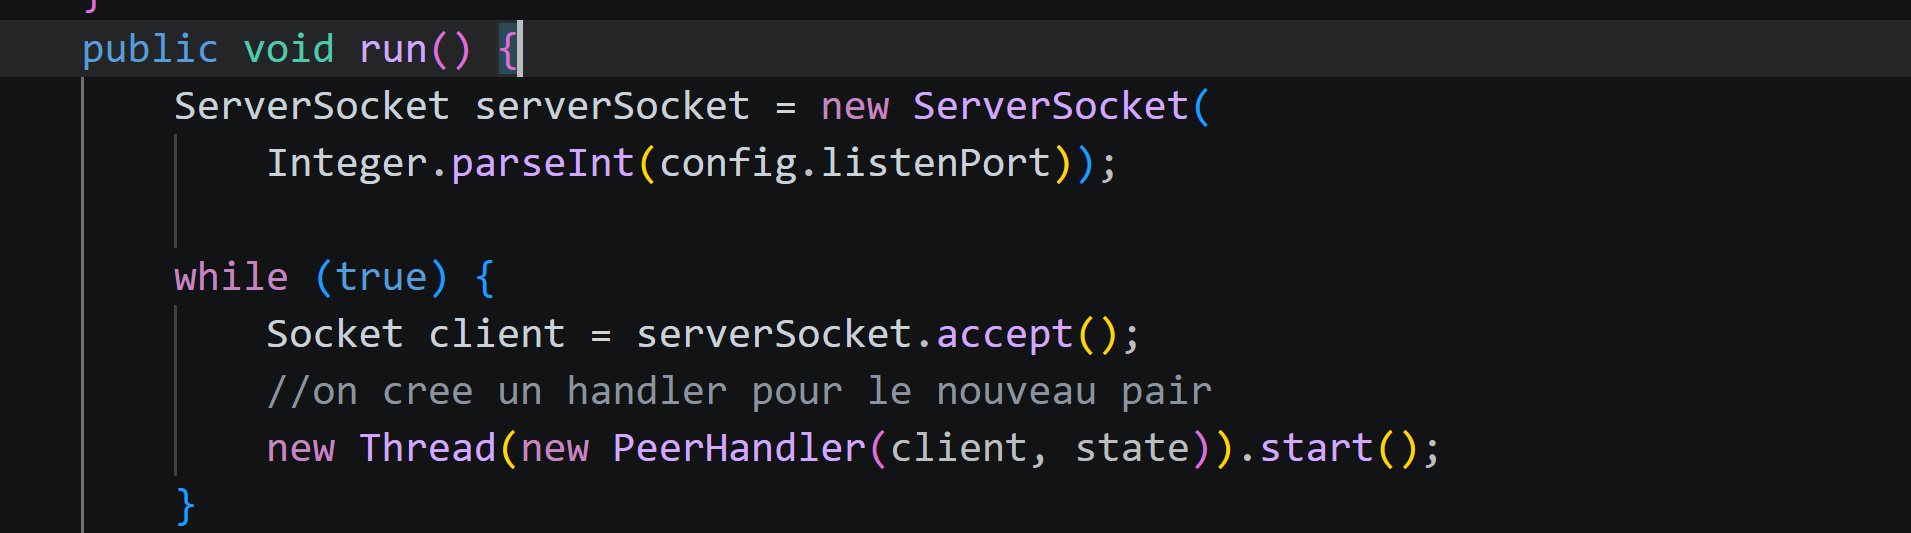
\includegraphics[width=0.7\linewidth]{peerserver.png}
    \caption{Architecture du PeerServer}
    \label{fig:peerserver}
\end{figure}

Cela permet de gérer plusieurs connexions simultanément.

\subsubsection{Gestion des commandes Peer-Peer}

Le \texttt{PeerHandler} gère plusieurs types de messages :

\paragraph{1. interested}
Lorsqu’un pair est intéressé par un fichier, il envoie :

\begin{verbatim}
interested <key>
\end{verbatim}

Le serveur répond avec un \textbf{buffermap} encodé en Base64.

\paragraph{2. have}
Cette commande permet d’échanger les buffermaps entre pairs.

Cela permet de savoir quelles pièces sont disponibles chez chaque voisin.

\paragraph{3. getpieces}
Le peer demande certaines pièces d’un fichier :

\begin{verbatim}
getpieces <key> [index1 index2 ...]
\end{verbatim}

Le serveur :
\begin{itemize}
    \item vérifie qu’il possède les pièces
    \item lit les données dans le fichier
    \item envoie un header + payload binaire
\end{itemize}

\subsubsection{Gestion du buffermap}

Le buffermap est représenté par un \textbf{BitSet} en Java.

\begin{itemize}
    \item 1 = pièce disponible
    \item 0 = pièce absente
\end{itemize}

Il est ensuite encodé en Base64 pour être transmis.

\subsubsection{Client Peer}

Le client permet de communiquer avec le tracker :

\begin{itemize}
    \item connexion TCP
    \item envoi de commandes (announce, look, getfile)
    \item réception des réponses
\end{itemize}

\subsubsection{Commande announce}

La commande announce permet d’envoyer la liste des fichiers au tracker.

Elle contient :
\begin{itemize}
    \item nom du fichier
    \item taille
    \item taille des pièces
    \item hash MD5
\end{itemize}

Le hash MD5 est calculé en lisant le fichier bloc par bloc.

\subsubsection{Points importants}

\begin{itemize}
    \item utilisation de TCP en mode flux
    \item séparation header / données binaires
    \item gestion des threads pour la concurrence
\end{itemize}

\section{Choix techniques}

\begin{itemize}
    \item Java pour le peer
    \item TCP pour la communication
    \item MD5 pour l’identification des fichiers
    \item Threads pour gérer plusieurs connexions
\end{itemize}

\section{Travail réalisé}

\begin{itemize}
    \item Implémentation du serveur peer
    \item Gestion des commandes réseau
    \item Encodage du buffermap en Base64
    \item Communication avec le tracker
\end{itemize}

\section{Difficultés rencontrées}

\begin{itemize}
    \item 
    \item 
    \item 
\end{itemize}

\section{Travail restant}

\begin{itemize}
    \item Optimisation du téléchargement
    \item Interface utilisateur
    \item Tests complets en réseau
\end{itemize}

\section{Conclusion}

Ce projet nous a permis de comprendre les principes fondamentaux des systèmes distribués 
et du protocole P2P. La suite du projet consistera à améliorer les performances 
et finaliser l’ensemble des fonctionnalités.

\end{document}